\section{Formulation}
The objective of this section is to show that the function $\sigma(x,y)$ used to represent the superficial bait density (kg/m$^2$), must comply with the following property
$$\int_{-\frac{w}{2}}^{+\frac{w}{2}} \sigma(x)dx=\frac{\dot{m}}{s},$$
where $\dot{m}$ is the bait flow (kg/s), $s$ is the speed of the helicopter (m/s), and $w$ is the swath width (m).

% Ambiente para incluir figura centrado, con pies de figuras y etiqueta para usar como referencia cruzada
\begin{figure}[h]
  \centering
  \includegraphics[width=120mm]{../resultados/png/helicopter-flight-path.png}
  \caption{Schematic of a helicopter’s flight path over a swath with three
  dispersal cells; $w$ is the swath width; $\delta y$ is the distance between two
  GPS points; and $A_{\mbox{cell}}$ is the area of a dispersal cell.}
  \label{fig:esquemaHelicoptero}
\end{figure}

We set the origin of a Cartesian coordinate system on the middle point of the
inferior side of a rectangle with base $w$ and height $\delta y$. This way, the
inferior side is found at $y=0$, the superior side at $y=\delta y$,the left side
at $x=-\frac{w}{2}$ and the right side at $x=+\frac{w}{2}$.

After the helicopter completes a pass, in each point $(x,y)$ of the rectangle a superficial bait density is obtained $\sigma(x,y)$. The definition of the superficial bait density of mass $m$ indicates that $\sigma(x,y)=\frac{dm}{dA}$. Rewriting the superficial density substituting $dA$ by $dydx$ and integrating along the dispersion cell, it follows that
% Ambiente para incluir ecuación y etiquetarla
\begin{equation}
  \delta m=\int_{-\frac{w}{2}}^{+\frac{w}{2}} \int_{0}^{\delta y} \sigma(x,y)dydx.
  \label{eq:masaEsIntegralDobleDeDensidad}
\end{equation}

\begin{figure}
  \centering
  % Ambiente para incluir subfigura
  \begin{subfigure}[b]{0.45\textwidth}
    
\includegraphics[width=\textwidth]{../resultados/png/constant-bait-density.png}
    \caption{Constant bait density along each swath.}
    \label{fig:densidadConstante}
  \end{subfigure}
  \begin{subfigure}[b]{0.45\textwidth}
    
\includegraphics[width=\textwidth]{../resultados/png/variable-bait-density.png}
    \caption{Variable bait density along each swath.}
    \label{fig:densidadVariable}
  \end{subfigure}
  \caption{
  Hypothetical island with bait swaths. Each green band represents one bait swath. The intensity of the bait swath color corresponds to its density, with darker colors indicating greater densities.
  }
\end{figure}


Assuming superficial density is uniform with respect to the helicopter’s flight
path, represented in Figure \ref{fig:densidadConstante}, equation \eqref{eq:masaEsIntegralDobleDeDensidad} becomes
\begin{equation}
  \frac{\delta m}{\delta y}=\int_{-\frac{w}{2}}^{+\frac{w}{2}}\sigma(x)dx.
  \label{eq:densidadLineal}
\end{equation}

The left-hand side of the equation represents the linear bait density which is
related with the mass flow of bait from the bucket and the speed of the
helicopter.  A helicopter equipped with a dispersion bucket with a constant mass
flow rate,
\begin{equation}
  \dot{m}=\frac{\delta m}{\delta t}
  \label{eq:flujoMasico}
\end{equation}
flies from the point $(0,0)$ to the point $(0,\delta y)$ with a speed of
\begin{equation}
  s=\frac{\delta y}{\delta t}.
  \label{eq:rapidez}
\end{equation}

Combining equations \eqref{eq:flujoMasico} and \eqref{eq:rapidez}, the linear bait
density
\begin{equation}
  \frac{\delta m}{\delta y}=\frac{\dot{m}}{s},
  \label{eq:densidadLinealEsflujoSobreRapidez}
\end{equation}
is obtained.

Finally, setting equations \eqref{eq:densidadLineal} and \eqref{eq:densidadLinealEsflujoSobreRapidez} equal to each other, we obtain
\begin{equation}
  \int_{-\frac{w}{2}}^{+\frac{w}{2}} \sigma(x)dx=\frac{\dot{m}}{s}.
  \label{eq:integralDeDensidadEsflujoSobreRapidez}
\end{equation}

Equation \eqref{eq:integralDeDensidadEsflujoSobreRapidez}  relates a density that is needed in the field with the variables of the bait dispersal mechanism.
